\documentclass{article}
\usepackage[T1]{fontenc}
\usepackage[utf8]{inputenc}
\usepackage{charter} 
\usepackage[charter]{mathdesign}  
\usepackage[table]{xcolor}   % For table rows coloring
\usepackage{listings}        % To show when calling multiGWAS from console

\usepackage{amsmath}         % For writhing p-values
\newcommand{\mathA}[1]{{\operatorname{#1}}}
\newcommand{\mathB}[1]{{\operatorname{\mathit{#1}}}}


\usepackage[active]{srcltx}
\usepackage{textcomp}
\usepackage{graphicx}
\usepackage{authblk}
\usepackage{lineno}
\usepackage{subfigure}
\usepackage{multicol}
\usepackage{float}
\usepackage{hyperref}
% debe ser en formato APA pero en overleaf es sin parentesis después reviso en local

%----Added by LuisG. References in a file exported from Mendeley---
\usepackage{biblatex}
\addbibresource{multiGWAS.bib}
%---------------------------------------------

\makeatother
\linenumbers
\begin{document}




\title{MultiGWAS: A tool for GWAS analysis on tetraploid organisms by integrating the results of four GWAS software}

\author[1]{L. Garreta}

\author[1]{I. Cer\'{o}n-Souza}
\author[2]{M.R. Palacio}
\author[1]{P.H. Reyes-Herrera}

\affil[1]{Corporaci\'{o}n Colombiana de Investigaci\'{o}n Agropecuaria (AGROSAVIA), CI Tibaitat\'{a},  Kil\'{o}metro 14, V\'{i}a a Mosquera, 250047, Colombia}

\affil[2]{Corporaci\'{o}n Colombiana de Investigaci\'{o}n Agropecuaria (AGROSAVIA), CI El Mira, Kil\'{o}metro 38, V\'{i}a Tumaco Pasto, Colombia}


\maketitle

%%226/250
%IAquí hice unos cambios pequeños para ampliar el espectro del estudio a cualquier planta tetraploide ya que esta revista está enfocada en herramientas para estudios evolutivos de cualquier organismo. Att. Ivania
\begin{abstract}
\textbf{Summary:} The Genome-Wide Association Studies (GWAS) are essential to determine the association between genetic variants across individuals. One way to support the results is by using different tools to validate the reproducibility of the associations. Currently, software for GWAS in diploids is well-established but for polyploids species is scarce. Each GWAS software has its characteristics, which can cost time and effort to use them successfully. Here, we present MultiGWAS, a tool to do GWAS analysis in tetraploid organisms by executing in parallel and integrating the results from four existing GWAS software: two available for polyploids (GWASpoly and SHEsis) and two frequently used for diploids (PLINK and TASSEL). The tool deals with all the elements of the GWAS process in the four software, including (1) the use of different control quality filters for the genomic data, (2) the execution of two GWAS models, the full model with control for population structure and individual relatedness and the Naive model without any control. The summary report generated by MultiGWAS provides the user with tables and plots describing intuitively the significant association found by both each one and across four software, which helps users to check for false-positive or false-negative results.\\
%PAULA: no se si explicamos un poco mejor el output acá?
\textbf{Contact:} phreyes@agrosavia.co\\

\textbf{Keywords: GWAS, tetraploids, SNPs,XXX}

\end{abstract}
\maketitle 

\section{Introduction}

%Ya está modificada la intro para incluir diferentes especies de plantas poliploides. Faltan las citas. Estoy haciendo una lista de referencias que hay que leer con calma. Especialmente reviews. Intentaré en los próximos días ampliarhttps://www.overleaf.com/project/5e8b8de6ae23ed0001a9a14f este primer párrafo conforme vaya leyendo las referencias que bajé. Pero el sentido general creo que ya quedó establecido. Att. Ivania 

The GWAS (Genome-Wide Association Study) is used to identify which variants through the whole genome of a large number of individuals are associated with a specific trait \cite{cantor2010prioritizing, begum2012comprehensive}. This methodology started with humans and several model plants, such as rice, maize, and $Arabidopsis$ \cite{lauc2010genomics, tian2011genome, cao2011whole, korte2013advantages, han2013sequencing}. Because of the advances in the next-gen sequencing technology and the decline of the sequencing cost in recent years, there is an increase in the availability of genome sequences of different organisms at a faster rate \cite{ekblom2011applications, ellegren2014genome}. Thus, the GWAS is becoming the standard tool to understand the genetic bases of either ecological or economic phenotypic variation for both model and non-model organisms. This increment in GWAS includes complex species such as polyploids (Fig \ref{GWASpolyploids}) \cite{ekblom2011applications, santure2018wild}. 

\begin{figure}
\begin{center}
%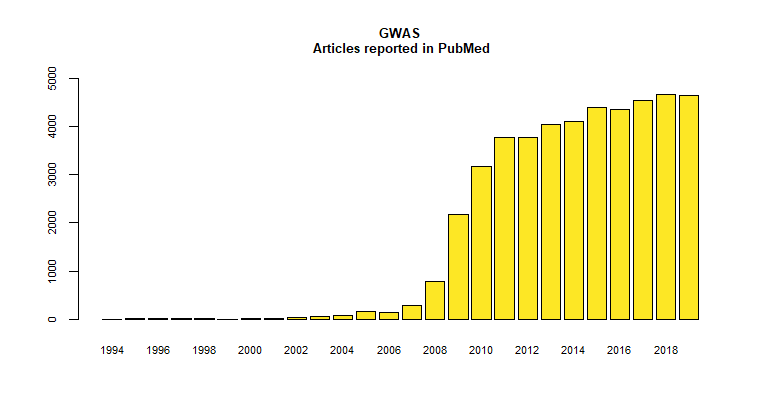
\includegraphics[width=13cm]{images/GWAStimeline.png}
    
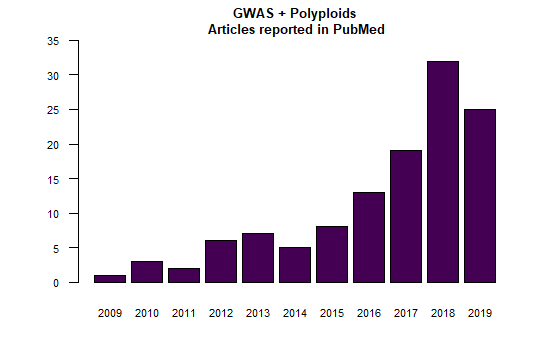
\includegraphics[width=12cm]{images/GWASpolyploids.png}

\caption{Timeline for articles reported for GWAS studies on polyploid species in PubMed. We present data for completed years.\label{GWASpolyploids}}
\end{center}

\end{figure}


The GWAS for polyploid species has three related challenges. First, as all GWAS, we should replicate the study as a reliable method to validate the results and recognize real associations. This replication involves finding the same associations either in several replicates from the study population using the same software or testing different GWAS tools among the same study population. This approach involved the use of different parameters, models, or conditions, to test how consistent the results are \cite{De2014,Pearson2008}. However, the performance of different GWAS software could affect the results. For example,  the threshold $pvalue$ for SNP significance change through four GWAS software (i.e., PLINK, TASSEL, GAPIT, and FaST-LMM) when sample size varies \cite{Yan2019}. It means that well-ranked SNPs from one package can be ranked differently in another.

Second, although there are many GWAS software available to repeat the analysis under different conditions \cite{Gumpinger2018}, most of them are designed exclusively for the diploid data matrix \cite{Bourke2018}. Therefore, it is often necessary to "diploidizing" the polyploid genomic data in order to replicate the analysis. 

Third, there are very few tools focused on the integration of several GWAS software, to make comparisons under different parameters and conditions across them. As far as we know, there is only two software with this service in mind, such as iPAT and easyGWAS. 

The iPAT allows running in a graphic interface three well-known command-line GWAS software such as GAPIT, PLINK, and FarmCPU (Chen and Zhang, 2018). However, the output from each package is separated. On the other hand, the easyGWAS allows running a GWAS analysis on the web using different algorithms. This analysis could run independently of both the computer capacity and operating system. However, it needs either several datasets available or a dataset with a large number of individuals to make replicates in order to compare among algorithms. Moreover, the output from different algorithms is separated \cite{Grimm2017}.  Thus, for both software iPAT and easyGWAS, the integrative and comparative outputs among software or algorithms are missing. 

To solve all the three challenges above, we developed the MultiGWAS tool that performs GWAS analyses for tetraploid species using four software in parallel. Our tool include GWASpoly \cite{Rosyara2016} and the SHEsis tool \cite{Shen2016} that accept polyploid genomic data, and PLINK \cite{Purcell2007} and TASSEL \cite{Bradbury2007} with the use of a "diploidized" genomic matrix. The tool deals with preprocessing data, running four GWAS tools in parallel, and create comparative reports from the output of each software to help the user to decide more intuitively the true or false associations.


\section{Method}

The MultiGWAS tool has three main steps: the adjustment stage, the multi analysis stage, and the integration step (Fig. \ref{pipeline}). In the first stage, MultiGWAS processes the configuration file. Then it cleans and filters the genotype and phenotype, and  MultiGWAS "diploidize" the genomic data. In the second stage, each GWAS tool runs in parallel. In the last stage, after the output files scanning, a summary of results is generated in a report that contains score tables, Venn diagrams, SNP profiles, and Manhattan plots. 

\begin{figure}
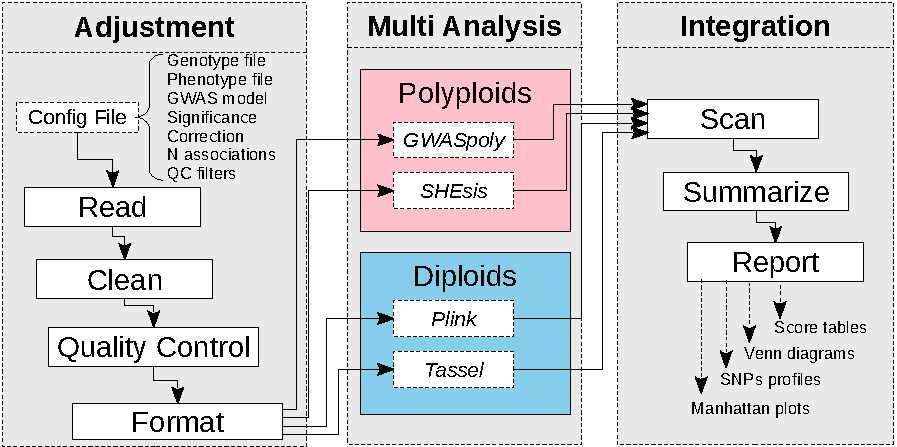
\includegraphics[width=12cm]{images/multi-gwas-flowchart-horizontal-stages-config.pdf}
\caption{MultiGWAS flowchart has three stages: adjustment, multi analysis, and integration.\label{pipeline}}

\end{figure}

\subsection{Adjustment stage} 

MultiGWAS takes as input a configuration file where the user specifies the genomics data along with the parameters that will be used by the four tools. Once the configuration file is processed, MultiGWAS preprocess the data that is cleaning, filtering, and checking data quality. The output of this stage corresponds to the inputs for the four programs at the Multi Analysis stage.



%genotype/phenotype filenames, genome-wide significance threshold, multiple testing correction methods, GWAS model, number of associations to be reported, and TRUE or FALSE whether to use quality control (QC) filters or not. 
 
% Preview source code from paragraph 15 to 17

% Preview source code from paragraph 15 to 17

\subsubsection{Configuration file}

The configuration file includes the following settings that we briefly describe:% (1) Input genotype and phenotype file names (2) GWAS model, (3) Significance threshold, (4) Correction (5) Quality Control (QC) filters and (6) number of associations to report. 

\paragraph{Input genotype and phenotype files:}

Currently, MultiGWAS uses two input files, one for genotype and the other for the phenotype. Both data correspond to data matrices with column and row names (Figure \ref{fig:File-Formats}). The genotype file uses SNP markers in rows and samples in columns (Figure \ref{fig:File-Formats}a). The phenotype file uses samples in rows and traits in columns (Figure \ref{fig:File-Formats}b) with the first column corresponding to the sample name and the second column to trait value.

%Paula: Luis una pregunta, recibimos solo formato ACGT? o recibimos otro formato??

\begin{figure}[H]
\begin{centering}
\begin{minipage}[t]{0.6\columnwidth}%
\begin{center}
\fbox{\begin{minipage}[t]{0.99\columnwidth}%

\scriptsize\textcolor{gray}{\texttt{Marker,Chrom,Pos,Indiv01,Indiv02,Indiv03,...}}
\texttt{c2\_41437,0,805179,AAAG,AAGG,AAGG,...}
\texttt{c2\_24258,0,1252430,AAGG,AGGG,GGGG,...}
\texttt{c2\_21332,0,3499519,TTCC,TTCC,TTCC,... }\\
\texttt{...}%
\end{minipage}}\\
a
\par\end{center}%
\end{minipage}~~~~~~~~~%
\begin{minipage}[t]{0.3\columnwidth}%
\begin{center}
\fbox{\begin{minipage}[t]{0.99\columnwidth}%
\scriptsize\textcolor{gray}{\texttt{Individual,Traitname}}

\texttt{Indiv01, 3.59}\\
\texttt{Indiv02, 4.07}\\
\texttt{Indiv03, 1.05}

\texttt{...}%
\end{minipage}}\\
b
\par\end{center}%
\end{minipage}
\par\end{centering}
\begin{centering}
\par\end{centering}
\caption{\textbf{MultiGWAS genotype and phenotype formats}. Both files are in CSV format (Comma Separated Values) and contain as first row the header labels of the columns. Although the header labels are arbitrary, the column order is obligatory. \textbf{a.} Genotype file format, where ``Marker'', ``Chrom'', and ``Pos'', correspond to the names for marker name, chromosome, and position in the first three columns respectively. The next columns correspond to the columns for the samples content. \textbf{b.} Phenotype file format, where ``Individual'' and ``Traitname'' are the column names for the individual and trait names, respectively.\label{fig:File-Formats}}
\end{figure}

\paragraph{GWAS model:}
MultiGWAS implements two types of GWAS analysis: (1) \textit{naive} and (2) \textit{full}. The \textit{naive} model without any control for structure or relatedness between samples (without any additional parameters). Whereas the \textit{full model}, known as the Q+K model, takes into account population structure (Q) and relatedness (K) to prevent false associations. We estimate Q and K inside MultiGWAS. 

Both models use linear regression. The \emph{naive} is modeled with Generalised Linear Models (GLMs, Phenotype + Genotype), and the \emph{full} is modeled with Mixed Linear Models (MLMs, Phenotype + Genotype + Structure + Kinship). The default model used by MultiGWAS is the \emph{full model} (Q+K) \cite{Yu2006}, which is described with the following equation:

\[
y=X\beta+S\alpha+Q\nu+Z\mu+e
\]

where $y$ is the vector of observed phenotypes; $\beta$ is a vector of fixed effects; $\alpha$ is a vector of SNP effects (Quantitative Trait Nucleotides); $\nu$ is a vector of population effects; $\mu$ is a vector of polygene background effects; $e$ is a vector of residual effects; $Q$, modeled as a fixed effect, refers to the incidence matrix for subpopulation covariates relating $y$ to $\nu$; and $X$, $S$ and $Z$ are incidence matrices of ones and zeros relating $y$ to $\beta$, $\alpha$ and $\mu$, respectively.

%Paula: QUantitavie trait nucleotides??? duda del termino


\paragraph{Genome-wide significance and multiple testing correction:}
GWAS searches SNPs associated with the phenotype in a statistically significant manner. A threshold or significance level $\alpha$ is specified and compared with the \emph{p-value} derived for each association score. Standard significance levels are 0.01 or 0.05 \cite{Gumpinger2018,Rosyara2016}.  However, due to the massive number of statistical tests performed by GWAS, the \emph{p-values }must be adjusted appropriately, performing a correction method for multiple hypothesis testing (MHT). 

MultiGWAS allows two MHT methods for adjusting \emph{p-values:} the Bonferroni correction and the false discovery rate (FDR). In the case of the Bonferroni correction, the threshold is $\alpha/m$, where \emph{m }is the number of valid markers from the genotype matrix (not missing or null values). (default $\alpha$=0.05, Correction=Bonferroni)

%Paula: Luis estos parámetro por default de QC y alpha faltan

\paragraph{Quality Control filters:}
A control step is necessary to check the input data for genotype or phenotype errors that can lead to spurious GWAS results.  MultiGWAS provides the filtering option (TRUE or FALSE) to check the input data by applying four quality control filters: Minor Allele Frequency
(MAF), individual missing rate (MIND), SNP missing rate (GENO), and Hardy\-Weinberg threshold (HWE). 

MAF of \{x\} filters out SNPs with minor allele frequency below \{x\} (default 0.01); MIND of \{x\} filters out all individuals with missing genotypes exceeding \{x\}{*}100\% (default 0.1); GENO \{x\} filters out SNPs with missing values exceeding \{x\}{*}100\% (default 0.1); and HWE filters out SNPs which have Hardy-Weinberg equilibrium exact test \emph{p-value} below the \{x\} threshold.

MultiGWAS does the MAF filtering. We use the PLINK package \cite{Gumpinger2018} for the other three filters: MIND, GENO, and HWE. Once we have the samples and SNPs that pass the filters, then we generate an input file for each package used. 

\paragraph{Number of best ranked associations:}
Criticism has arisen in considering only statistically significant associations as the only possible correct associations \cite{Thomson2011,Kaler2019}. Many of low \emph{p-value} associations, closer to being significant, are discarded due to the stringent significance levels, and consequently increasing the number of false negatives. To help to analyze both significant and non-significant associations, MultiGWAS provides the option to specify the number of best-ranked associations, adding the corresponding  \emph{p-value} to each association found.  In this way, it is possible to enlarge the number of results, and we can observe replicability in the results for different programs. Nevertheless, we present each association with the corresponding \emph{p-value}.%  We present the resultant associations in different tables and graphics reported by MultiGWAS (see Figure \ref{fig:-View-Shared-SNPs}). 




\subsubsection{Data preprocessing}
Once the configuration file is processed, then the genomic data is preprocessed by selecting individuals present in both genotype and phenotype and excluding individuals and SNPs that have poor quality. Moreover, the format   "ACGT" suitable for the polyploid software GWASpoly and SHEsis, is "diploidized" for PLINK and TASSEL. The homozygous tetraploid genotypes are converted to diploid thus: (e.g.,AAAA\textrightarrow AA, CCCC\textrightarrow CC, GGGG\textrightarrow GG,
TTTT\textrightarrow TT). Moreover, for tetraploid heterozygous genotypes, the conversion depends on the reference and alternate alleles calculated for each position (e.g., AAAT\textrightarrow AT,
... ,CCCG\textrightarrow CG). After this process, MultiGWAS transform the genomic data into the formats required for each software.



\subsection{Multi analysis stage} 

%\subsubsection{Tools}
We have selected four GWAS software tools to be integrated into our multiGWAS tool. Two designed specifically for polyploid species: GWASpoly \cite{Rosyara2016} and SHEsis \cite{Yong2006}. Another two designed for diploids species and extensively used in humans and plants: PLINK \cite{Purcell2007,Chang2015} and TASSEL \cite{Bradbury2007}, respectively. We briefly describe each tool as follows.

%MultiGWAS runs in parallel using two types of statistical models specified in the parameters file, the Full model (Q+K) and Naive (i.e., without any control) \cite{Sharma2018}. The Full model (Q+K) controls for both population structure and individual relatedness. For population structure, MultiGWAS uses the Principal Component Analysis (PCA) and takes the top ten PC as covariates. For relatedness, the tool uses kinship matrices that TASSEL and GWASpoly calculated separately, and for PLINK and SHEsis depends on the King software \cite{Manichaikul2010}. 

As MultiGWAS implements two types of GWAS analysis,  \emph{naive} and  \emph{full}, each tool is called in two different ways.
%The naive without any additional parameter, but the full with two parameters that take into account for population structure (Q) and relatedness (K) to prevent false associations.

\subsubsection{GWASpoly}

GWASpoly \cite{Rosyara2016} is an R package designed for GWAS in polyploid species used in several studies in plants \cite{Berdugo2017,Ferrao2018,Sharma2018,Yuan2019}. GWASpoly uses a Q+K linear mixed model with biallelic SNPs that account for population structure and relatedness. Also, to calculate the SNP effect for each genotypic class, GWASpoly provides a general gene action model along with four additional models: additive, simplex dominant, and duplex dominant. We use all the models to find associations.

MultiGWAS is using GWASpoly version 1.3. The population structure and relatedness, used in the \emph{full} model, are estimated using the first five principal components and the kinship matrix, respectively, both calculated with the algorithms built-in GWASpoly.  


\subsubsection{SHEsis}

SHEsis \cite{Shen2016} is a program written in C designed for polyploid species. It includes single locus association analysis, among others. It is based on a linear regression model, and it has been used in some studies of animals and humans \cite{Qiao2015,Meng2019}. 

MultiGWAS is using version 1.0, which does not take account for population structure or relatedness. However, MultiGWAS externally estimates relatedness for SHEsis by excluding individuals with cryptic first-degree relatedness using the algorithm implemented in PLINK 2.0 (see below).


\subsubsection{PLINK}

PLINK \cite{Purcell2007} is a program written in C frequently used in diploids species in particular humans \cite{Power2016}. PLINK includes univariate GWAS using two-sample tests and linear regression models.

MultiGWAS is using two versions of PLINK: 1.9 and 2.0. We use the linear regression from PLINK 1.9 to achieve both types of analysis, \emph{naive} and \emph{full}. We use the first five principal components calculated with the PLINK 1.9 built-in algorithm to estimate the population structure. We estimate the relatedness from the kinship coefficients calculated with the PLINK 2.0 built-in algorithm, removing the close relatives or individuals with the first-degree relatedness.

\subsubsection{TASSEL}

TASSEL  \cite{Bradbury2007}  is a GWAS program written in Java, frequently used for diploid plant studies. TASSEL was developed for maize data \cite{Alvarez2017,Zhang2018}. For association analysis, TASSEL includes the general linear model (GLM) and mixed linear model (MLM) that accounts for population structure and relatedness.

MultiGWAS is using TASSEL 5.0. The \emph{naive} GWAS uses GLM. The \emph{full} GWAS uses MLM with two parameters: one for population structure, using the first five principal components, and another for relatedness, using the kinship matrix with centered IBS method, both calculated with the TASSEL built-in algorithms.


\subsection{Integration stage.} The outputs resulting from the four software are scanned and processed to identify both significant and best-ranked associations. MultiGWAS corrects (correction method defined in the configuration file) the p-values and calculates the threshold value for each associated marker. The calculation uses the number of valid genotype calls (i.e., non-missing genotypes, phenotypes, and covariates). 

\begin{figure}

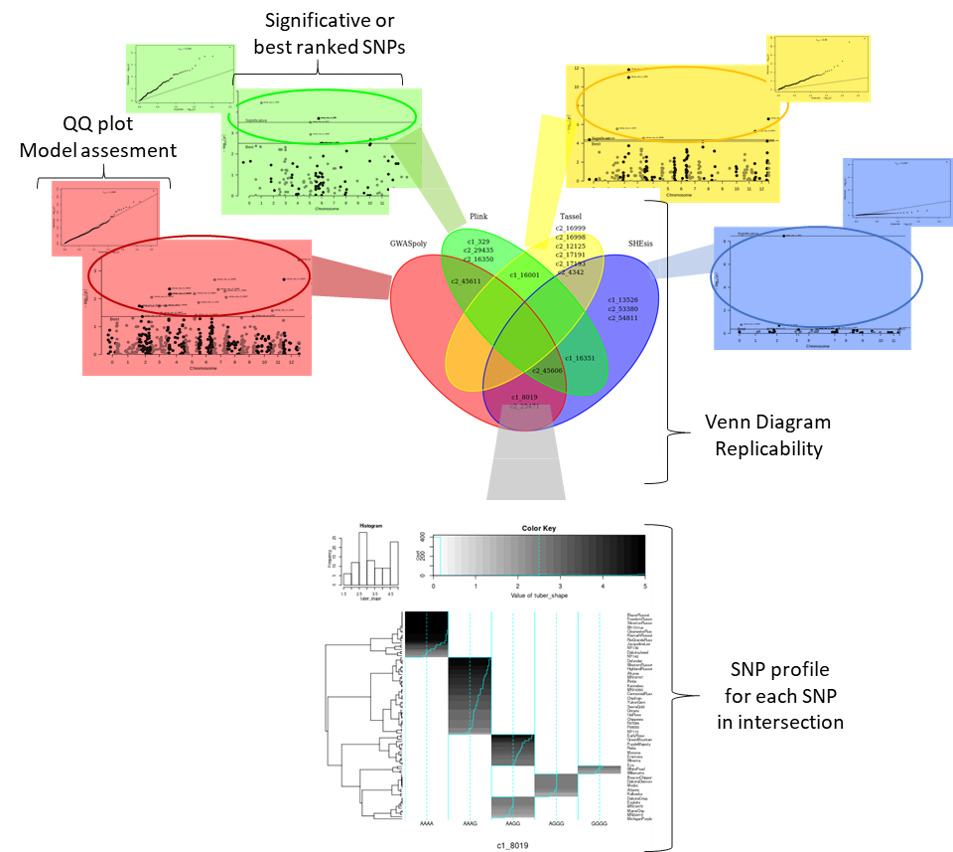
\includegraphics[width=15cm]{images/Reportes_Metodologia.png}
\caption{We present several reports. For each tool, first a QQ plot that asses the resultant p-values.  Second, a Manhattan plot for each tool with two lines, blue and red, respectively, is the lower limit for the best ranked and significative SNPs. We present two Venn diagrams, one for the significative SNPs and one for N best-ranked SNPs of each tool. We show the results for GWAspoly, PLINK, TASSEL, and SHEsis in red, green, yellow, and blue, respectively. Moreover, for each SNP that is in the intersection; thus, that is predicted by more than one tool we provide SNP profile. \label{reports}}
\label{pipeline}
\end{figure}

At this stage, We integrate the results to evaluate reproducible results among tools (Fig \ref{reports}). But, We still report a summary for the results of each tool:
\begin{itemize}
    \item A Quantile-Quantile (QQ) plots for the resultant p-values of each tool and the corresponding degree of inflation $\lambda$ to asses the degree of the test statistic inflation.
    \item AA Manhattan plot of each tool with two lower thresholds, one for the best-ranked SNPs, and another for the significant SNPs. 
\end{itemize}

To present the replicability, we use two sets: (1) the set of all the significative SNPs provided by each tool and (2) the set of all the best-ranked SNPs. For each set, we present a Venn diagram that shows SNPs predicted exclusively by one tool and intersections that help to identify the SNPs predicted by one, two, three, or all the tools. In addition, we provide detailed tables for the two sets.

For each SNP predicted more than once, we provide what we call the SNP profile. That is a heat diagram for a specific SNP, where each column is a genotype state AAAA, AAAB, AABB, ABBBB, BBBBB. And each row corresponds to a sample. Samples with close genotypes form together clusters. Thus to generate the clusters, we do not use the phenotype information. However, we present the phenotype information in the figure as the color. This figure visually provides information regarding genotype and phenotype information simultaneously for the whole population. We present colors as tones between white and black for color blind people. 


MultiGWAS generates a report, one document with the content previously described. Besides, there is a folder with the individual figures just in case the user needs one. In the supplementary information, we include a report and a description of the report content\textcolor{red}{(supplementary information XXX)}

%PAula: infomración suplementary con reporte completo y figuras. Y explicación del reporte

In the following section, we present the results applied to a public dataset. 





\section{Results}
% Preview source code from paragraph 27 to 29

Although most of the GWAS packages used by MultiGWAS use linear regression approaches, they often produce different association results for the same input. For example, computed \emph{p-values }for the same set of SNPs are different between packages; SNPs with significant \emph{p-values} for one package maybe not significant for the others, or well-ranked SNPs in one package may be ranked differently in another. To alleviate these difficulties, MultiGWAS produces four types of outputs using different graphics and tabular views, including score tables, Venn diagrams, Manhattan and Q-Q plots, and SNP profiles. We designed these outputs to help users visually to compare, select, and interpret the set of possible SNPs associated with a trait of interest. 

As an example of the functionality of the tool, here we show the results of running MultiGWAS tool in the genomic data from a tetraploid potato diversity panel, genotyped and phenotyped as part of the USDA-NIFA Solanaceae Coordinated Agricultural Project (SolCAP) \cite{Hirsch2013}. The reports include: significant SNPs, best-ranked SNPs, profile SNPs, and visualization of associations. First, the best-ranked SNPs (Figure \ref{fig:-View-Shared-SNPs}.b), where the SNP c2\_45606 was evaluated with a high score by the four packages, but other four SNPs were also ranked with high scores by two packages simultaneously. Second, the significant SNPs (Figure \ref{fig:-View-Shared-SNPs}.c), where the two polyploid software, GWASpoly and SHEsis, found as significant three SNPs, c1\_8019, c2\_25471, and c2\_45606. In particular, the c1\_8019 was also the most significant association found in the same potato dataset analyzed by Rosyara et al. (2016). 

For each SNPs identified by more than one package, we provide the SNP profile (Figure \ref{fig:SNP-profiles}), where for each significant association, a heat map figure is generated to summarize the genotype associated with a trait for each individual. Here we present, the SNP profile for the SNPs ranked among the best for the four tools c2\_45606. We also include the SNP profile for the  c1\_8019 the most significant SNP for both polyploid tools. The SNP profiles for the markers present in the intersections are in the \textcolor{red}{(supplementary information XXX)}


And fourth, the visualization of associations (Figure \ref{fig:view-qqmanhattan}), where for each package, a Manhattan and QQ plots are generated using special marks to help to identify significative, best-ranked, and shared SNPs (found by more than one tool). 



% Figure Manhattan and QQ plots
\begin{figure}[H]
\noindent %
\noindent\begin{minipage}[t]{1\columnwidth}%
\begin{minipage}[t][1\totalheight][c]{0.5\columnwidth}%
\begin{center}
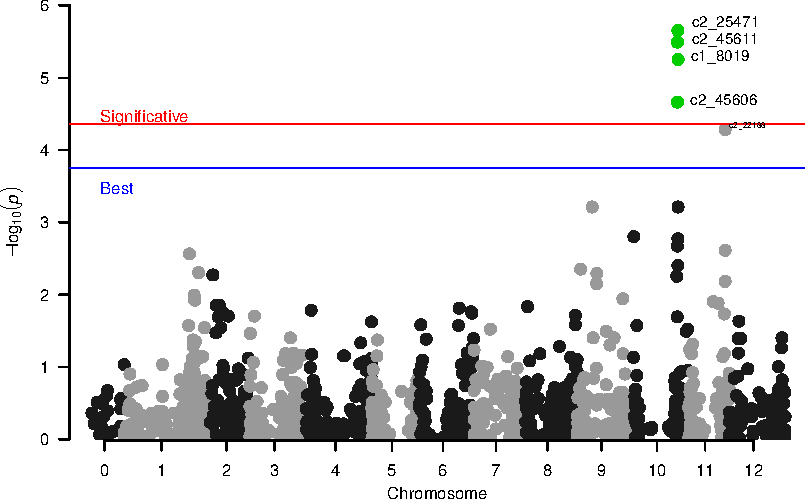
\includegraphics[scale=0.5]{images/out-multiGWAS-views-manhattan-GWASpoly}\\
(a)
\par\end{center}%
\end{minipage}%
\begin{minipage}[t][1\totalheight][c]{0.5\columnwidth}%
\begin{center}
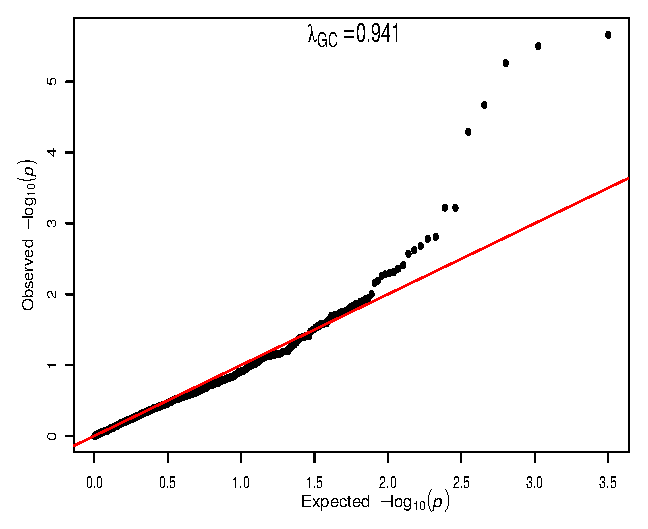
\includegraphics[bb=-30bp 0bp 294bp 238bp,clip,scale=0.5]{images/out-multiGWAS-views-QQ-GWASpoly}\\
(b)
\par\end{center}%
\end{minipage}%
\end{minipage}

\caption{\scriptsize\textbf{MultiGWAS visualization of associations.} MultiGWAS adds special marks to the Manhattan and QQ plots to help identify different types of SNPs: (a) In Manhattan plots, significant SNPs are above a red line, best-ranked SNPs are above a blue line, and shared SNPs (See Figure \ref{fig:-View-Shared-SNPs}.b) are colored in green (b) In QQ plots, a red diagonal line indicates the expectation, so potential associations can be observed when the number of SNPs deviating from the diagonal is small, as in the case of monogenic traits, or when this number is somewhat higher, as in the case of truly polygenic traits. However, deviations for a high number of SNPs could reflect inflated \emph{p-values }owing to population structure or cryptic relatedness. \label{fig:view-qqmanhattan}}
\end{figure}


The complete report from MultiGWAS for the naive and full model is in the Supplementary information (\href{https://github.com/agrosavia-bioinformatics/multiGWAS}{https://github.com/agrosavia-bioinformatics/multiGWAS}) 




\subsection{Visualization of shared SNPs}
GWAS packages rely on \emph{p-value }as a measure of association between each individual SNP and the trait of interest. The SNPs are considered statistically significant, and so possible true associations, when their \emph{p-value }falls below a predefined significance level, usually 0.01 or 0.05. But, most GWAS packages compute differently both \emph{p-values }and significance levels, it could result in non-significant SNPs. Consequently, it is important to know the significant SNPs. It is equally important to know the best-ranked SNPs closer to being statistically significant, as they may represent important associations to consider for posterior analysis (e.g. false negatives).

MultiGWAS provides tabular and graphic views to report in an integrated way both the best-ranked and significant SNPs identified by the four GWAS packages (see Figure \ref{fig:-View-Shared-SNPs}). Both \emph{p-values} and significance levels have been scaled as $-log_{10}(\mathB{p-value})$ to give high scores to the best statistically evaluated SNPs.
%PAULA: será que ponemos el pvalue? como la gente esta acostumbrada. 


First, the best-ranked SNPs correspond to the top-scored \emph{N} SNPs that are the ones corresponding to the N lower p-values. \ref{fig:-View-Shared-SNPs}.a) and in a Venn diagram (Figure \ref{fig:-View-Shared-SNPs}.b). The table lists them by package and sorts by decreasing score, whereas the Venn diagram shows them emphasizing if these ones were best-ranked either in a single package or in several at once (shared). And second, the significant SNPs correspond to the ones assesed statistically significant by each package (depending on the threshold), they are shown in a Venn diagram (Figure \ref{fig:-View-Shared-SNPs}.b), and they are also shown in the SNPs table, marked with significance TRUE and score greater than threshold, columns SGN, SCR, and THR, respectively in the table of the Figure\ref{fig:-View-Shared-SNPs}.a.


%PAULA:(1) en esta tabla falta c2\_45606 para tassel. (2) El THR todavía me confunde a mi, prque varia para cada método?

% Figure SNPs table and Venn diagrams
\begin{figure}[H]
{\fboxrule 0.2pt\fbox{\begin{minipage}[t][1\totalheight][b]{0.46\columnwidth}%
\renewcommand{\arraystretch}{1.5}
\setlength{\tabcolsep}{0.2em}
\rowcolors{2}{gray!25}{white}
\tiny
\begin{center}
\begin{tabular}{cccccccc}
\hline 
PKG & MDL & CHR & POS & SNP & SCR & THR & SGN\tabularnewline
\hline 
GWASpoly & Full & 10 & 48863165 & c1\_8019 & 4.78 & 4.25 & TRUE\tabularnewline
GWASpoly & Full & 10 & 48808404 & c2\_25471 & 4.57 & 4.27 & TRUE\tabularnewline
GWASpoly & Full & 10 & 48203431 & c2\_45611 & 4.36 & 4.27 & TRUE\tabularnewline
GWASpoly & Full & 10 & 48218826 & c2\_45606 & 4.68 & 4.5 & TRUE\tabularnewline
GWASpoly & Full & 4 & 71591813 & c2\_10692 & 2.93 & 4.25 & FALSE\tabularnewline
GWASpoly & Full & 4 & 71592285 & c2\_10687 & 2.93 & 4.25 & FALSE\tabularnewline
GWASpoly & Full & 4 & 71827521 & c2\_10614 & 2.93 & 4.25 & FALSE\tabularnewline
PLINK & Full & 10 & 67293176 & c1\_16001 & 1.7693 & 3.2601 & FALSE\tabularnewline
PLINK & Full & 10 & 77351069 & c1\_329 & 1.1795 & 3.301 & FALSE\tabularnewline
PLINK & Full & 11 & 51404231 & c2\_29435 & 1.1188 & 3.2553 & FALSE\tabularnewline
PLINK & Full & 10 & 69323144 & c2\_45611 & 1.0229 & 3.2553 & FALSE\tabularnewline
PLINK & Full & 2 & 41814861 & c2\_16350 & 0.9598 & 3.301 & FALSE\tabularnewline
PLINK & Full & 10 & 69311500 & c2\_45606 & 0.8489 & 3.2923 & FALSE\tabularnewline
PLINK & Full & 10 & 69809843 & c1\_16351 & 0.6131 & 3.2833 & FALSE\tabularnewline
SHEsis & Full & 2 & 13697423 & c1\_8019 & 9.4711 & 3.301 & TRUE\tabularnewline
SHEsis & Full & 1 & 30837971 & c1\_13526 & 8.4501 & 3.2923 & TRUE\tabularnewline
SHEsis & Full & 5 & 46046095 & c2\_53380 & 8.2409 & 3.2601 & TRUE\tabularnewline
SHEsis & Full & 3 & 39255236 & c2\_25471 & 7.8241 & 3.2923 & TRUE\tabularnewline
SHEsis & Full & 5 & 49804489 & c2\_54811 & 6.9633 & 3.2695 & TRUE\tabularnewline
SHEsis & Full & 1 & 69809843 & c1\_16351 & 6.0247 & 3.2833 & TRUE\tabularnewline
SHEsis & Full & 4 & 69311500 & c2\_45606 & 5.9557 & 3.2923 & TRUE\tabularnewline
TASSEL & Full & 8 & 54838024 & c2\_16999 & 3.6076 & 3.8943 & FALSE\tabularnewline
TASSEL & Full & 8 & 54838005 & c2\_16998 & 3.483 & 3.8943 & FALSE\tabularnewline
TASSEL & Full & 1 & 71450400 & c2\_12125 & 2.4832 & 3.8943 & FALSE\tabularnewline
TASSEL & Full & 1 & 70474651 & c2\_17191 & 2.45 & 3.8943 & FALSE\tabularnewline
TASSEL & Full & 1 & 70472380 & c2\_17193 & 2.2893 & 3.8943 & FALSE\tabularnewline
TASSEL & Full & 10 & 47539878 & c1\_16001 & 2.9101 & 4.5512 & FALSE\tabularnewline
TASSEL & Full & 7 & 14924207 & c2\_4342 & 2.8793 & 4.5512 & FALSE\tabularnewline
\hline 
\end{tabular}
\par\end{center}
\begin{center}
\normalsize (a)
\par\end{center}%
\end{minipage}}}~~~~~~~~~~~%
\noindent\begin{minipage}[t]{1\columnwidth}%
{\fboxrule 0.2pt\fboxsep 2pt\fbox{\begin{minipage}[t][1\totalheight][c]{0.38\columnwidth}%
\begin{center}
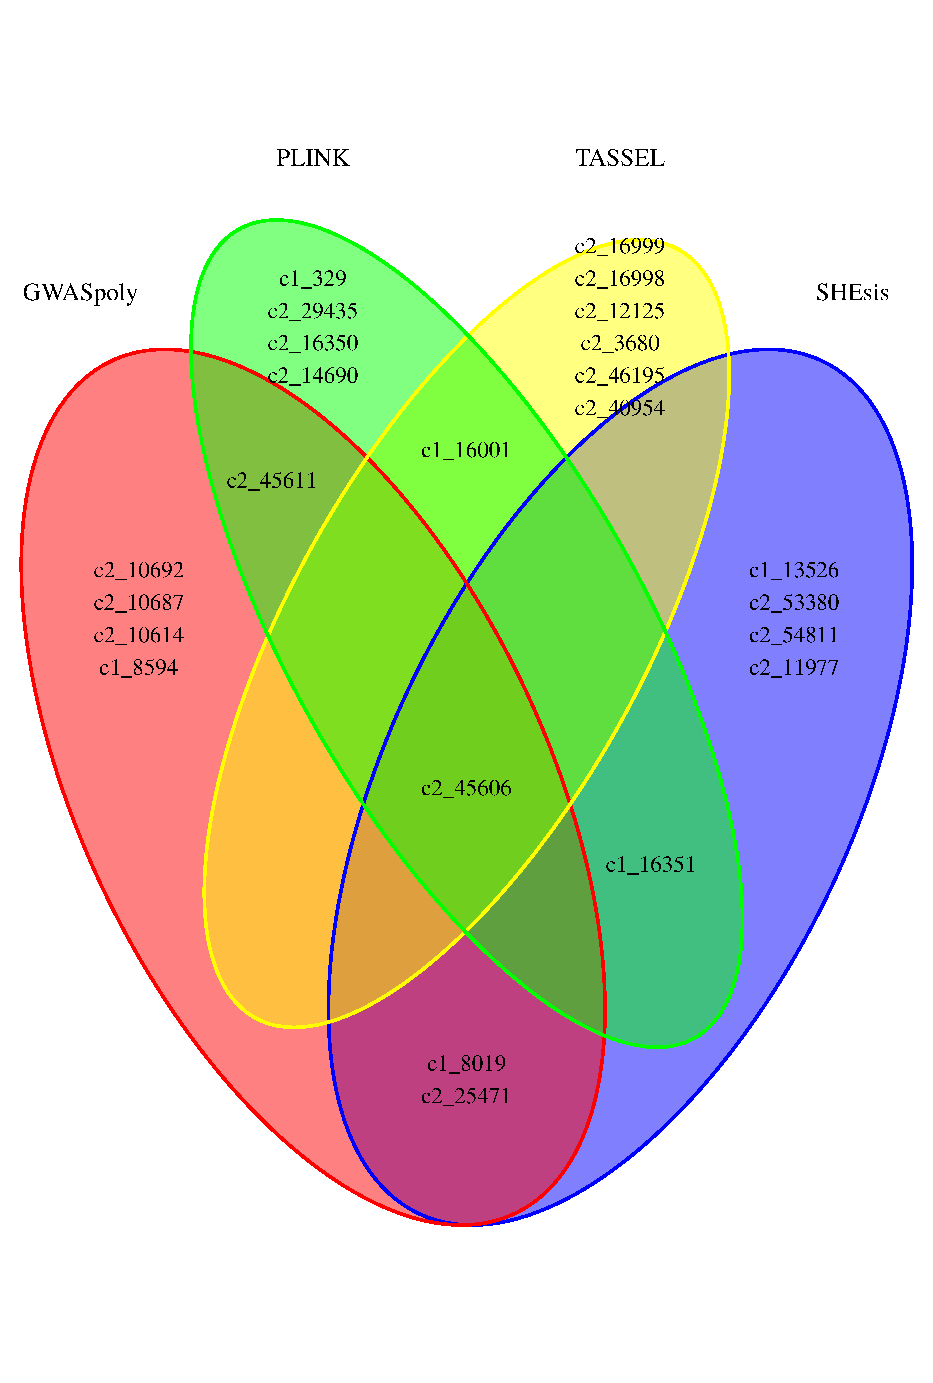
\includegraphics[bb=0bp 60bp 432bp 590bp,clip,scale=0.25]{images/out-multiGWAS-vennDiagram-best}\\
(b)
\par\end{center}%
\end{minipage}}}

~

{\fboxrule 0.2pt\fboxsep 2pt\fbox{\begin{minipage}[t][1\totalheight][c]{0.38\columnwidth}%
\begin{center}
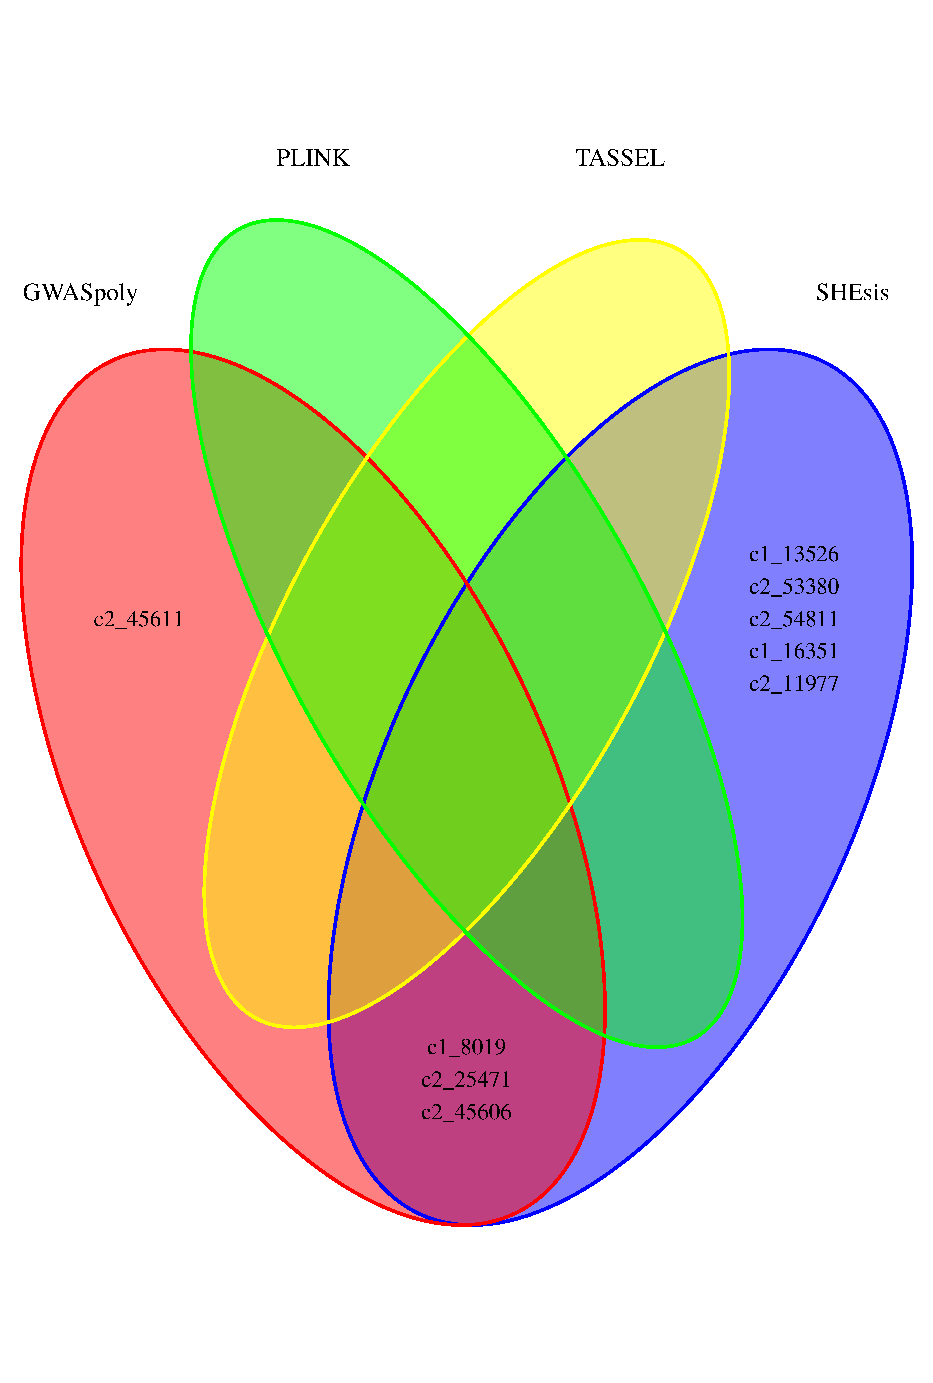
\includegraphics[bb=0bp 60bp 432bp 590bp,clip,scale=0.25]{images/out-multiGWAS-vennDiagram-significatives}\\
(c)
\par\end{center}%
\end{minipage}}}%
\end{minipage}
\begin{centering}
\par\end{centering}
\caption{\scriptsize \textbf{Visualization of shared SNPs.} Tabular and graphical views of the best-ranked and significant SNPs identified by the four packages. \textbf{(a)} Tabular view with detailed information of each SNPs, including: package name (PKG), GWAS model used (MDL), chromosome (CHR), position in the genome (POS), ID (SNP), score (SCR), threshold (THR), and significance flag (SGN), wether the SNP was evaluated statistically significant or not (score > theshold). \textbf{(b)} Venn diagram with the best-ranked SNPs, showing that one SNP was shared by the four packages (c2\_45606), other two only by the two polyploid packages GWASpoly and SHEsis (c1\_8019 and c2\_25471), and other one only by the two diploid packages PLINK and TASSEL (c1\_16001). \textbf{(c)} Venn diagram with the significant SNPs, showing that only three SNPs (c1\_8019, c2\_25471, and c2\_45606) were evaluated as significant by the two polyploid packages GWASpoly and SHEsis.\label{fig:-View-Shared-SNPs}}
\end{figure}



\subsection{Visualization of shared SNPs}
MultiGWAS creates a two-dimensional representation, what we called SNP profile, to visualize each trait by individuals and genotypes as rows and columns, respectively (Figure \ref{fig:SNP-profiles}). At the left, the individuals are grouped in a dendrogram by their genotype. At the right, there is the name or ID of each individual. At the bottom, the genotypes are ordered from left to right, starting from the major to the minor allele (i.e., AAAA, AAAB, AABB, ABBB, BBBB). At the top, there is a description of the trait based on a histogram of frequency (top left) and by an assigned color for each numerical phenotype value using a grayscale (top right). Thus, each individual appears as a colored line by its phenotype value on its genotype column. For each column, there is a solid cyan line with the mean of each column and a broken cyan line that indicates how far the cell deviates from the mean.

Because each multiGWAS report shows one specific trait at a time, the histogram and color key will remain the same for all the best-ranked SNPs.

% Figure SNP profiles
\begin{figure}[H]
\noindent\begin{minipage}[t]{1\columnwidth}%
\begin{minipage}[t]{0.5\columnwidth}%
\begin{center}
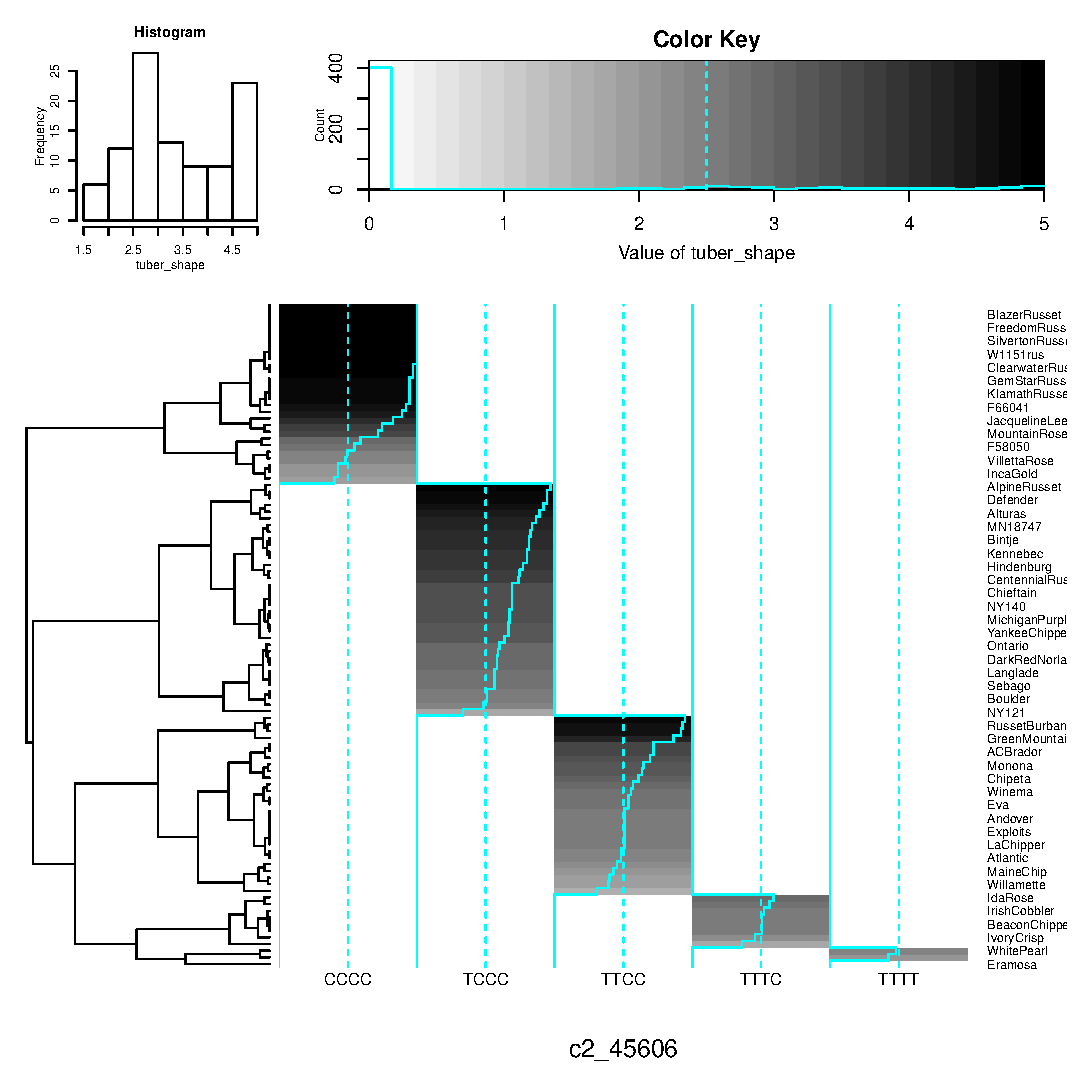
\includegraphics[scale=0.3]{images/out-SNPProfile-c2_45606}\\
(a)
\par\end{center}%
\end{minipage}%
\begin{minipage}[t]{0.5\columnwidth}%
\begin{center}
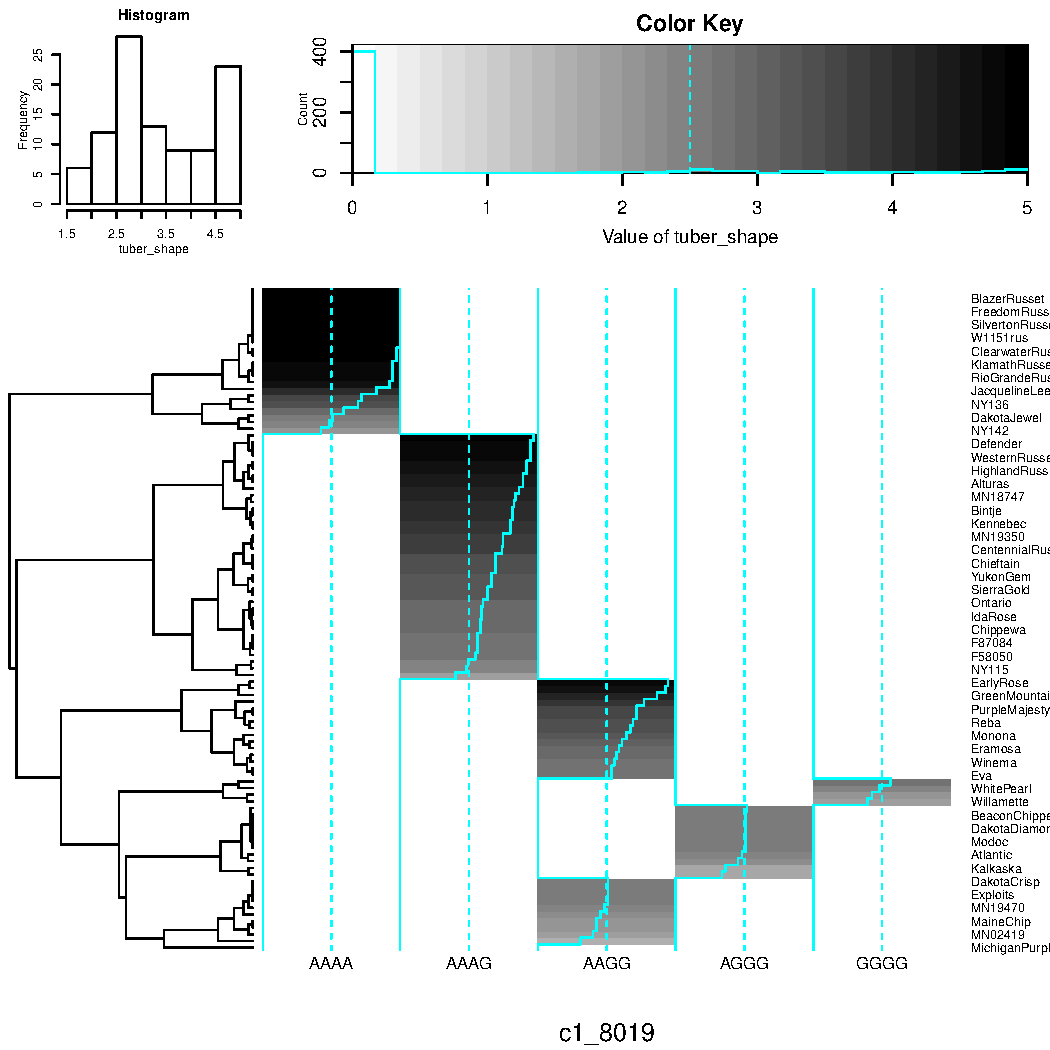
\includegraphics[scale=0.3]{images/out-SNPProfile-c1_8019}\\
(b)
\par\end{center}%
\end{minipage}%
\end{minipage}

\caption{\textbf{\scriptsize{}SNP profiles. }{\scriptsize{}SNP profiles for two of the best-ranked significant SNPs shown in the figure \ref{fig:-View-Shared-SNPs}.b. (a) SNP c2\_45606 best-ranked by the four packages (central intersection of the Venn diagram Figure \ref{fig:-View-Shared-SNPs}.b) (b) SNP c1\_8019 best-ranked by the two tetraploid packages (Figure \ref{fig:-View-Shared-SNPs}.b), and also identified as significant by the same packages (at the bottom of the Figure \ref{fig:-View-Shared-SNPs}.a). \label{fig:SNP-profiles}}}
\end{figure}


%PAULA: el color key de ambos SNP profile esta mal, y tengo dudas de los colores de la imagen.

\section{Availability and implementation:} 
The core of the MultiGWAS tool was developed in R and users can interact with the tool by either a command line interface (CLI) developed in R or a graphical user interface (GUI) developed in Java (Figure \ref{fig:MultiGWAS-interaction}). Source code, examples, documentation and installation instructions are available at \href{https://github.com/agrosavia-bioinformatics/multiGWAS}{https://github.com/agrosavia-bioinformatics/multiGWAS}. 

\subsection{Input parameters}
MutiGWAS uses as the only input a simple configuration text file where users set the values for the main parameters that drives the GWAS process. The input parameters include: the output folder where results will be written, input genotype/phenotype filenames, genome-wide significance threshold, method for multiple testing correction, GWAS model, number of associations to be reported, and TRUE or FALSE whether to use quality control filters or not. The filters are: minor allele frequency, individual missing rate, SNP missing rate, and Hardy-Weinberg threshold.

The configuration file can be created either using a general text editor or using the GUI application. In the first case, the file must have the structure shown in the Figure \ref{fig:MultiGWAS-interaction}.a, where parameter names and values are separated by colon, filenames are enclosed in quotation marks, and TRUE or FALSE indicates wheter filters are applied or not. Moreover examples for the config file \href{https://github.com/agrosavia-bioinformatics/MultiGWAS/tree/master/examples}{https://github.com/agrosavia-bioinformatics/MultiGWAS/tree/master/examples}

In the second case, the user creates the config file in a simple and straightforward way using the input parameter view from the GUI application (Figure \ref{fig:MultiGWAS-interaction}.b) and clicking the ``Save'' button.


\subsection{Using the command line interface}

The execution of the tool in command line is simple, it only needs to open a linux console, change to the folder where the configuration file was created, and type the name of the executable tool followed by the filename of the configuration file, like this:

\begin{lstlisting}[language=bash,basicstyle={\small}]
multiGWAS full.config
\end{lstlisting}

Then, the tool starts the execution, showing information of the process in the console window, and when it finishes the results are saved to a new subfolder called \emph{``outgwas/reports}. Results include a full html report containing the different views described in the results section, along with the original graphics and summary tables created by MultiGWAS and used to create the html report. Additionally, results include the preprocessed tables of the main outputs generated by the four GWAS packages used by MultiGWAS.

\subsection{Using the graphical user interface}
The MultiGWAS GUI application can be executed either by running from a Linux console the \emph{jmultiGWAS} command or by clicking on the Java application file \emph{JMultiGWAS.jar} located in the \emph{``multiGWAS/sources''} subfolder. After it opens, it shows a main frame with four tabs at the top (Figure \ref{fig:MultiGWAS-interaction}b): ``Inputs'', ``Outputs'', ``Results'', and ``Files''. The ``Inputs'' tab shows the form to create the configuration file and run the application. The ``Outputs'' tab shows the messages from the running process after it starts the execution. The ``Results'' tab shows the full html report described above. And the ``Files'' tab shows an embedded file browser pointing to the subfolder that contains the original files used in the html report and described above.

\begin{figure}[H]
\begin{centering}
\begin{minipage}[t][1\totalheight][c]{0.5\columnwidth}%
\begin{center}
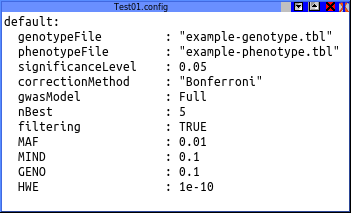
\includegraphics[scale=0.5]{images/screenshot-configFile}\\
(a)
\par\end{center}%
\end{minipage}
\par\end{centering}
~

~
\begin{centering}
\noindent\begin{minipage}[t]{1\columnwidth}%
\begin{center}
 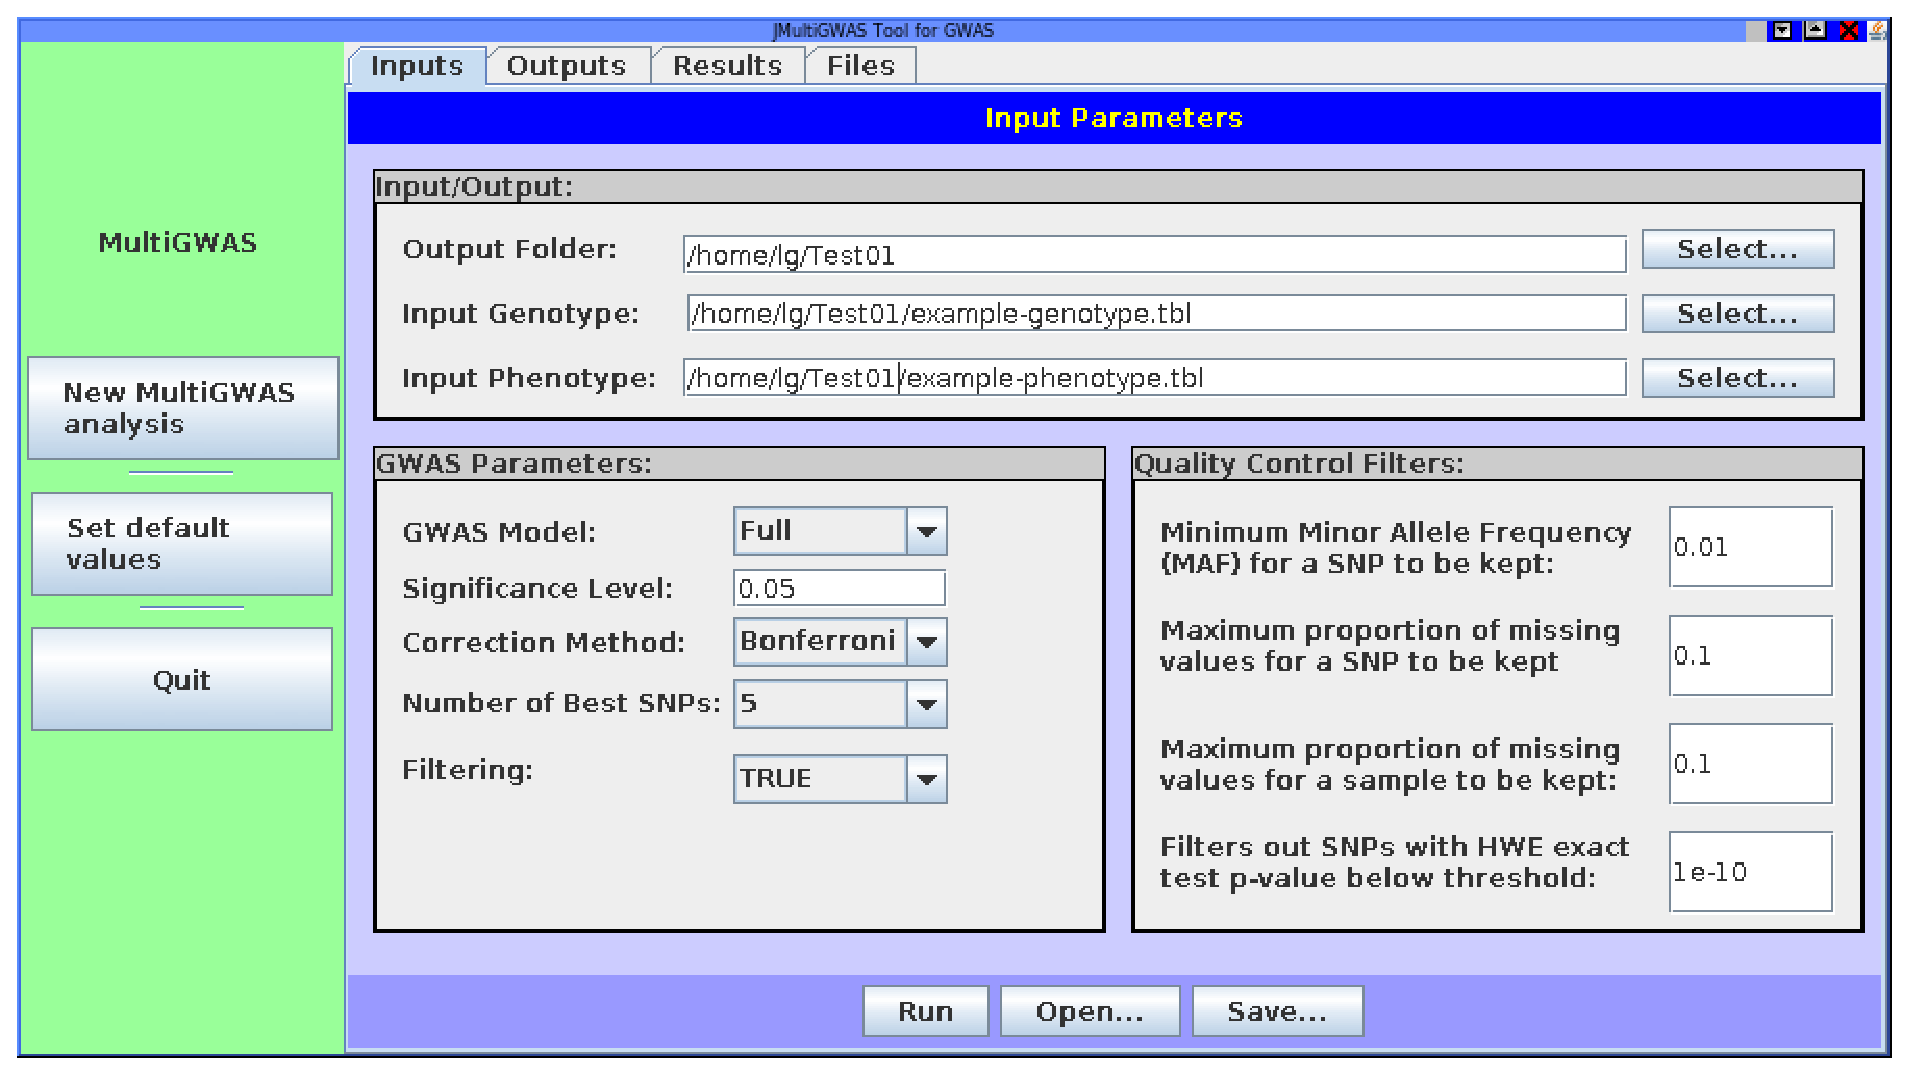
\includegraphics[scale=0.38]{images/screenshot-jmultiGWAS-inputsView}\\
(b)
\par\end{center}%
\end{minipage}
\par\end{centering}
\caption{\scriptsize\textbf{MultiGWAS inputs and interaction}. MultiGWAS uses as input a simple configuration text file and can be executed using either a command line interface script in R (CLI) or a graphic user interface application in Java (GUI). \textbf{(a) }An example of a configuration text file named \emph{``Test01.config'' }including the parameters that drive the GWAS process. It can be created using a general text editor or using the GUI application (see below) \textbf{(b) }Main view of the MultiGWAS GUI application (``Inputs'' view) where users can create the configuration file by setting values for input parameters. The GUI contains other three views: ``Outputs'' view shows the logs of the running process. ``Results'' view shows a report in html format with the tabular and graphics described in the results section. And, the ``Files'' view shows an embedded file manager pointing to the subfolder that contains the files created by MultiGWAS and used to create the report. \protect \\
\label{fig:MultiGWAS-interaction}}
\end{figure}

















\section{Discussion}
%PAULA: Falta discutir un tris los resultados a nivel de informaicón
%PAULA: Tools diploides vs Tools poliploides en poliploides 
XXXXXXXXXXXXXXXXXXXXXXX

%Also, the two diploid software, PLINK, and TASSEL identify a new marker, the c1\_16001. 



\printbibliography
% La bibliografia la coloqué toda en un archivo aparte "multiGWAS.bib" creado desde Mendeley y voy a compartirlerle un repositorio de Mendeley para que coloquen la bibliografía allá de forma más fácil y solo se exporte el archivo ("multiGWAS.bib") y se suba acá a overleaf (Yo puedo hacer eso)

\end{document}
